\documentclass[a4paper,11pt,fleqn]{scrartcl}%fleqn pour aligner les equations à gauche
\usepackage{../../Styles/Exercice}


\newcommand{\chnum}{Chapitre 21}
\newcommand{\chtitle}{Étude de la dynamique d'un système électrique}
\newcommand{\dtype}{Exercices}


\begin{document}
	\maketitle
\begin{multicols}{2}
\section{Estimer l'intensité d'un courant de charge}
Lors de la charge ultrarapide du bus \emph{Watt system} à l'aéroport de Nice, une charge d'environ \SI{100}{\kilo\coulomb} est transférée dans les super condensateurs du bus pendant une durée record de \SI{10}{\second}.\\
Estimer l'intensité $I$ du courant électrique supposée constante pendant la charge.

\section{Charger un condensateur à courant constant}
%\begin{minipage}{.6\linewidth}
La charge d'un condensateur se fait avec un courant d'intensité constante $I$ = \SI{0,010}{\mA}. La représentation graphique de l'évolution de la tension $u_C$ aux bornes du condensateur est donnée ci-contre.
%\end{minipage}
\begin{center}%{.4\linewidth}
	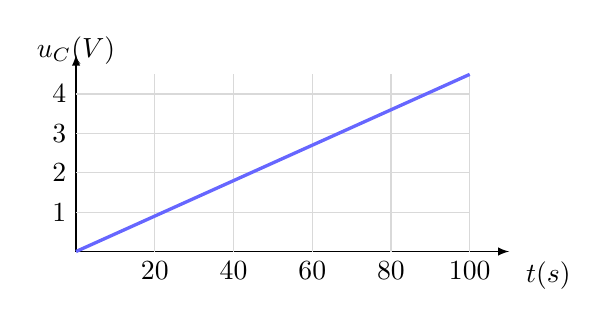
\begin{tikzpicture}[scale=.5]
		\draw[-latex] (0,0) to (0,5);
		\draw[-latex] (0,0) to (11,0);
		\foreach \k in {1,...,4}{
			\draw[gray!30] (0,\k) to (10,\k);
			\node[left] at (0,\k)  {\k};}
		\foreach \k in {2,4,...,10}{
			\draw[gray!30] (\k,0) to (\k,4.5);
			\node[below] at (\k,0)  {\k 0};}
		\draw [domain=0:10,samples = 600,blue!60,line width = 1.2pt] plot (\x,{0.45*\x});%courbe
		
		\node[above] at (0,4.5)  {$u_C (V)$};
		\node[below] at (12,0)  {$t (s)$};
		
	\end{tikzpicture}
\end{center}
\begin{enumerate}
	\item Donner l'expression de la charge $q(t)$ stockée dans le condensateur à la date $t$ en fonction de $t$ et de $I$.
	\item En déduire l'expression de la tension $u_C$ en fonction de $I$, $t$ et de la capacité $C$ du condensateur.
	\item Déterminer la valeur de la capacité $C$ du condensateur en \unit{\micro\farad}.
\end{enumerate}

\section{Décharge d'un condensateur}
%\begin{minipage}{.7\linewidth}
	Une lampe de poche dynamo comporte un super condensateur que l'on charge rapidement en tournant la manivelle. Lorsque le condensateur est complètement chargé, la tension à ses bornes vaut $U_0$ = \SI{3,6}{\volt}.\\
	On étudie la décharge du condensateur de capacité $C$ = \SI{1,0}{\farad} à travers une résistance $R$ = \SI{330}{\ohm}. À $t$ = \SI{0}{\second}, on ferme l'interrupteur $K$ et la décharge débute.
%\end{minipage}
\begin{center}%{.3\linewidth}
	 \begin{circuitikz}[scale=1.3]
		\draw (0,0)
		to [nos,l=$K$] ++(2,0)
		to [short] ++ (0,-2)
		to [R,v^>=$u_R$] ++ (-2,0)
		to [C,v^>=$u_C$,i<=$i$] ++(0,2)
		-- (0,0);
		\foreach \k in {-.3,-.1,.1,.3}{\node[above] at (\k,-.9){\footnotesize +}; \node[above] at (\k,-1.4){\footnotesize -};}
	\end{circuitikz}	
\end{center}
\begin{enumerate}
	\item Établir l'équation différentielle vérifiée par $u_C(t)$ pendant la décharge et montrer qu'elle peut s'écrire sous la forme $\dfrac{du_C}{dt}+\dfrac{1}{\tau}\cdot u_C =0$ où $\tau = RC$ est le temps caractéristique du circuit.
	\item Montrer que $u_C(t)=U_0\cdot e^{-\dfrac{t}{\tau}}$ est la solution de l'équation différentielle précédente.
	\item En déduire que le condensateur est presque complètement déchargé au bout d'une durée de l'ordre de \SI{30}{\minute}.
\end{enumerate}

\section{Étudier la charge d'un condensateur pour déterminer sa capacité}
% \begin{minipage}{.5\linewidth}
Un binôme d'élèves souhaite mesurer la valeur maximale de la capacité $C$ d'un condensateur ajustable.\\
Le condensateur est associé en série avec une résistance $R$ = \SI{1,0}{\mega\ohm}, un interrupteur et un générateur de tension continue $E$ = \SI{5,0}{\volt} avec acquisition informatisée de données.\\
Lors de la charge du condensateur, les élèves obtiennent le résultat ci-contre.
% \end{minipage}
\begin{center}%{.5\linewidth}
	%\centering
	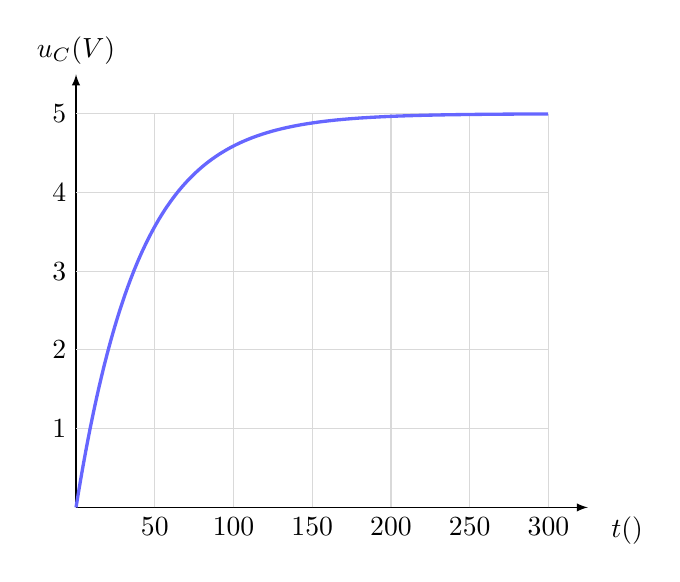
\begin{tikzpicture}
		\draw[-latex] (0,0) to (0,5.5);
		\draw[-latex] (0,0) to (6.5,0);
		\foreach \k in {1,...,5}{
			\draw[gray!30] (0,\k) to (6,\k);
			\node[left] at (0,\k)  {\k};}
		\foreach \k in {1,...,6}{
			\draw[gray!30] (\k,0) to (\k,5);
			\node[below] at (\k,0)  {\pgfmathparse{int(round(50*\k))} \pgfmathresult};}
		\draw [domain=0:6,samples = 600,blue!60,line width = 1.2pt] plot (\x,{5*(1-exp(-\x/0.8))});%courbe
		
		\node[above] at (0,5.5)  {$u_C (V)$};
		\node[below] at (7,0)  {$t (\unit{\micro\second})$};
		
	\end{tikzpicture}
\end{center}
\begin{enumerate}
	\item Déterminer par deux méthodes différentes la valeur du temps caractéristique $\tau$ du dipôle $RC$.
	\item En déduire la valeur maximale de la capacité $C$ du condensateur réglable et commenter le résultat.
\end{enumerate}

\section{Défibrillateur cardiaque}
La tension aux bornes d'un condensateur dans un défibrillateur cardiaque est de \SI{1,5}{\kilo\volt}. Lors du choc électrique produit sur le thorax du patient, la charge transférée est de \SI{0,30}{\coulomb}. On supposera que le condensateur est totalement déchargé après ce choc.
\begin{enumerate}
	\item Calculer la capacité $C$ du condensateur utilisé.
	\item Sachant que le thorax peut être modélisé par un conducteur ohmique de résistance $R$ = \SI{75}{\ohm}, estimer la durée du choc.
\end{enumerate}

\section{Temporisation d'une alarme}
Après avoir mis sous tension l'alarme d'un appartement il faut pouvoir disposer d'une durée suffisante pour sortir dans la déclencher. Pour cela, certains dispositifs utilisent la charge et la décharge d'un condensateur. Le circuit de l'alarme est alimenté par une batterie de tension à vide $E$ et de résistance interne négligeable. Le schéma simplifié du circuit électrique de l'alarme est le suivant :\\
%\begin{minipage}{.3\linewidth}
\textbf{Données} : \begin{itemize*}
	\item $R$ = \SI{47}{\ohm}
	\item $C$ = \SI{1,1}{\milli\farad}
	\item $E$ = \SI{9,0}{\volt}
\end{itemize*}
%\end{minipage}
\begin{center}%{.5\linewidth}
	
	\begin{circuitikz}[scale=.8, transform shape]
		\draw(0,0)
		to [nos,l=$K$] ++(2,0)
		to [R] ++ (2,0)
		to [short,-*] ++ (1,0)
		to [C, l=$C$] ++ (0,-2)
		to [short,-*] ++ (0,0)
		to [short] ++ (-5,0)
		to [battery2,v=$E$] ++ (0,2)
		--(0,0);
		\draw[dashed] (5,0)--(8,0);
		\draw[dashed] (5,-2)--(8,-2);
		\node[above] at (5,0){A};
		\node[below] at (5,-2){B};
		\node[above] at (8.5,-1.5)[text width=4cm] {Circuit de commande de la sirène};
	\end{circuitikz}
\end{center}

La mise sous tension de l'alarme correspond à la fermeture de l'interrupteur $K$. Le circuit de commande de la sirène est tel qu'à la fermeture de la porte de l'appartement, le condensateur est mis en court-circuit (ses armatures sont alors reliées par un fil conducteur non représenté sur le schéma).
	\textbf{Étude de la charge du condensateur dans le circuit RC}\\
	%\begin{minipage}{.5\linewidth}
		Pour étudier la charge du condensateur de capacité $C$, on enregistre l'évolution de la tension $u_{AB}=f(t)$ entre ses bornes à l'aide d'une interface d'acquisition reliée à un ordinateur. Le circuit de commande de la sirène n'est pas relié au condensateur lors de cette expérience. L'acquisition commence lors de la fermeture de l'interrupteur $K$, le condensateur étant préalablement déchargé. La courbe $u_{AB}=f(t)$ obtenue est représentée ci-dessous.
	%\end{minipage}
	\begin{center}%{.5\linewidth}
		%\centering
		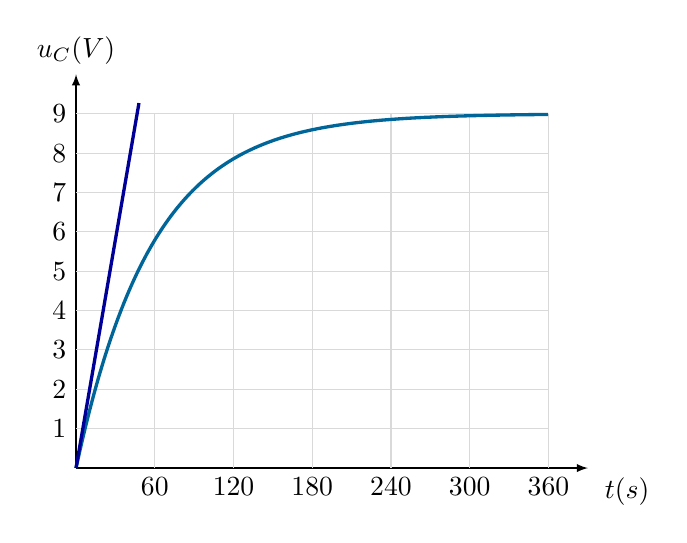
\begin{tikzpicture}
			\draw[-latex] (0,0) to (0,5);
			\draw[-latex] (0,0) to (6.5,0);
			\foreach \k in {0.5,1,...,4.5}{
				\draw[gray!30] (0,\k) to (6,\k);
				\node[left] at (0,\k)  {\pgfmathparse{int(round(2*\k))} \pgfmathresult};}
			\foreach \k in {1,...,6}{
				\draw[gray!30] (\k,0) to (\k,4.5);
				\node[below] at (\k,0)  {\pgfmathparse{int(round(60*\k))} \pgfmathresult};}
			\draw [domain=0:6,samples = 600,blue!60!green,line width = 1.2pt] plot (\x,{4.5*(1-exp(-\x/0.97))});%courbe
			\draw [domain=0:.8,samples = 600,blue!60!black,line width = 1.2pt] plot (\x,{5.8*\x});%tangente
			
			\node[above] at (0,5)  {$u_C (V)$};
			\node[below] at (7,0)  {$t (s)$};
			
		\end{tikzpicture}
	\end{center}
	\begin{enumerate}
		\item Reproduire le schéma du montage et indiquer les branchements de l'interface pour visualiser $u_{AB}=f(t)$.
		\item Déterminer la valeur de temps caractéristique $\tau$ de ce circuit et vérifier que cette valeur est en accord avec les caractéristiques du circuit.
	\end{enumerate}
	\textbf{Déclenchement de l'alarme}\\
	Ce circuit commande une sirène qui se déclenche dès que la tension aux bornes du condensateur atteint la valeur de \SI{8,0}{\volt}.
	\begin{enumerate}
		\item À l'aide de la courbe $u_{AB}=f(t)$ donnée, déterminer la durée $\Delta t$ dont dispose l'habitant pour quitter l'appartement et fermer la porte.
		\item Expliquer pourquoi le fait de fermer la porte empêche l'alarme de se déclencher.
	\end{enumerate}

\section{Machine de Wimhurst}
La machine de Wimhurst se comporte comme un condensateur d'une capacité de l'ordre de \SI{200}{\pico\farad}. Lorsque sa charge électrique est de l'ordre de \SI{2}{\micro\coulomb} et que l'écartement entre les boules de l'éclateur est d'environ \SI{1}{\centi\meter}, il se produit une étincelle.\\
Calculer, en $V$, l'ordre de grandeur de la tension aux bornes de l'éclateur juste avant l'étincelle.
\end{multicols}

\section{Un accéléromètre pour sauver des vies}
Un accéléromètre est un capteur qui, fixé à un mobile ou tout autre objet, permet de mesurer l'accélération de ce dernier dans une direction donnée.\\
Les accéléromètres capacitifs sont des systèmes à réponse très rapides en raison de la faible inertie de la partie mobile. L'une des premières applications de ce type de capteurs a été la détection de chocs appliquée au déclenchement du gonflage des airbags des véhicules.

\noindent \begin{minipage}[8cm]{.47\linewidth}
	\textbf{Document 1 : Fonctionnement de l'accéléromètre capacitif et déclenchement d'airbag}\\
	Un accéléromètre capacitif comporte un condensateur à capacité variable constitué de pièces en forme de peignes complémentaires qui constitue ses armatures. L'une est fixe et constitue le cadre. En cas de choc brutal du véhicule, la partie mobile se déplace dans le sens du mouvement, comme le passager d'un bus qui est debout et se trouve projeté en avant quand le bus freine. Ce changement de distance entre le peigne mobile et le cadre modifie la capacité du condensateur. Un circuit électrique associé à un microcontrôleur permet de détecter ce changement de capacité et de commander le gonflage de l'airbag, avant même que le condensateur et les passagers du véhicule ne soient projetés en avant.\\
	
	\centering 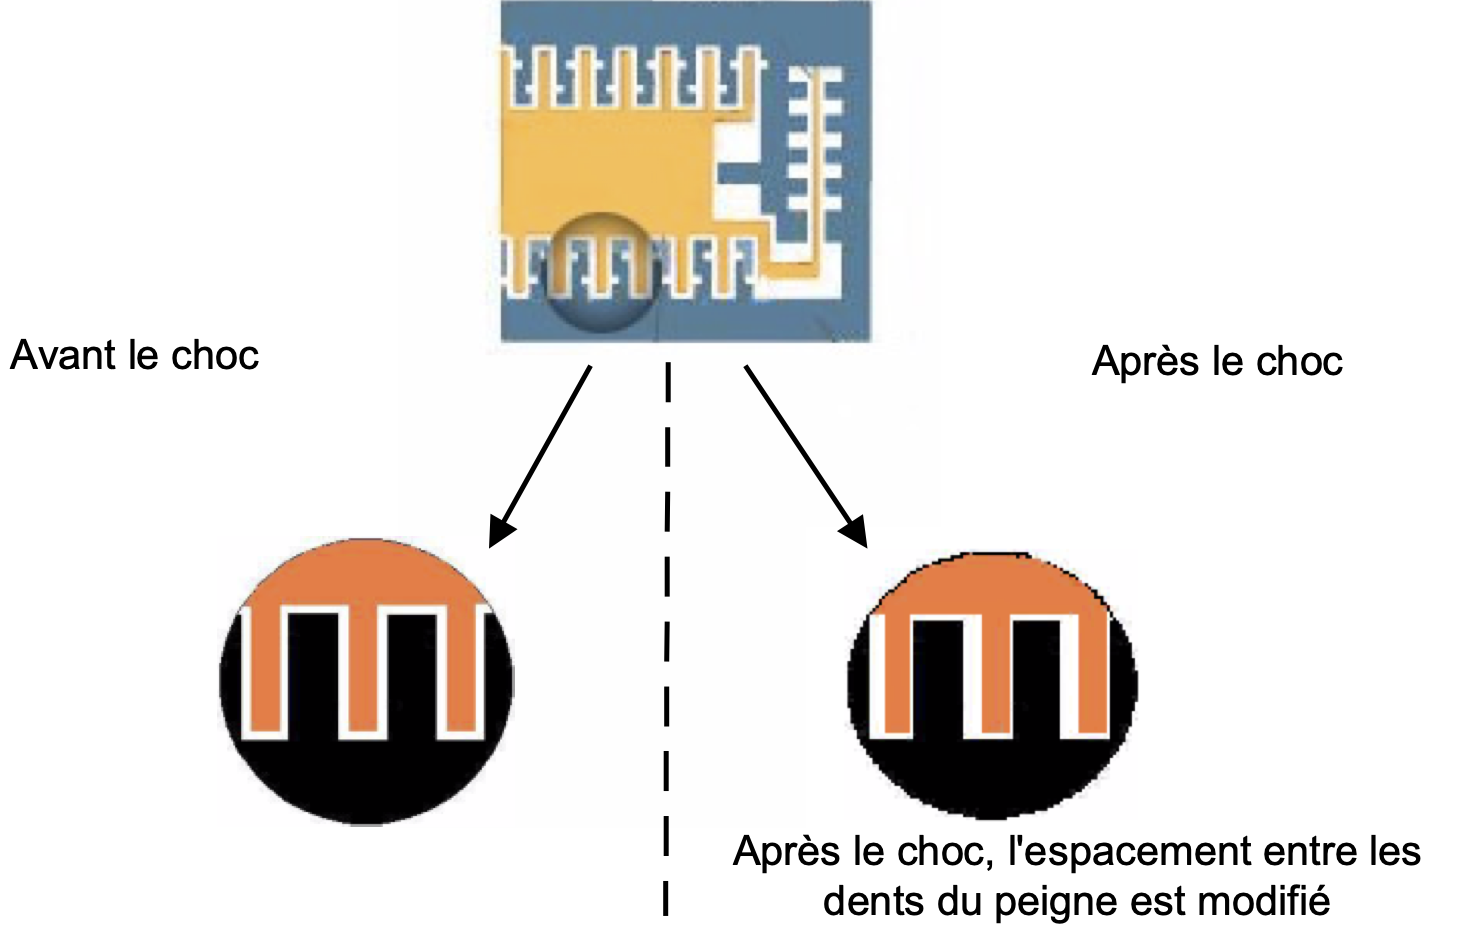
\includegraphics[scale=.6]{Ressources/TSPE_C11_Exercices_Fig2.png}	
\end{minipage}
\hspace{1em}
\begin{minipage}{.47\linewidth}
	\begin{minipage}{\linewidth}
	\textbf{Document 2 : Schéma du circuit de l'accéléromètre}\\
	Le peigne mobile et le cadre constituent un condensateur de capacité $C$. Il est branché aux bornes d'une pile de résistance interne $R$ et de force électromotrice $E$.\\
	En dehors d'un choc, lorsque l'accéléromètre est au repos : $C$ = \SI{100}{\pico\farad} ; $E$ = \SI{5,0}{\volt}.
	
	\centering\begin{circuitikz}
		\draw(0,0)
		to [nos,l=$K$] ++(2,0)
		to [C,i=$i$,v=$u_C$,l=$C$] ++ (2,0)
		to [short] ++ (2,0)
		to [short] ++ (0,-2)
		to [R, l=$R$] ++ (-4,0)
		to [vsource,v=$E$] ++ (-2,0)
		--(0,0);
		\node[below] at (0.45,-2)  {+};	
		\node[below] at (1.55,-2.1)  {-};	
		\node[below] at (2.5,.5)  {$q$};	
	\end{circuitikz}
	\end{minipage}
	\begin{minipage}{\linewidth}
		\textbf{Document 3 : Rapprochement des deux armatures du condensateur lors d'un choc}\\
		
		\centering 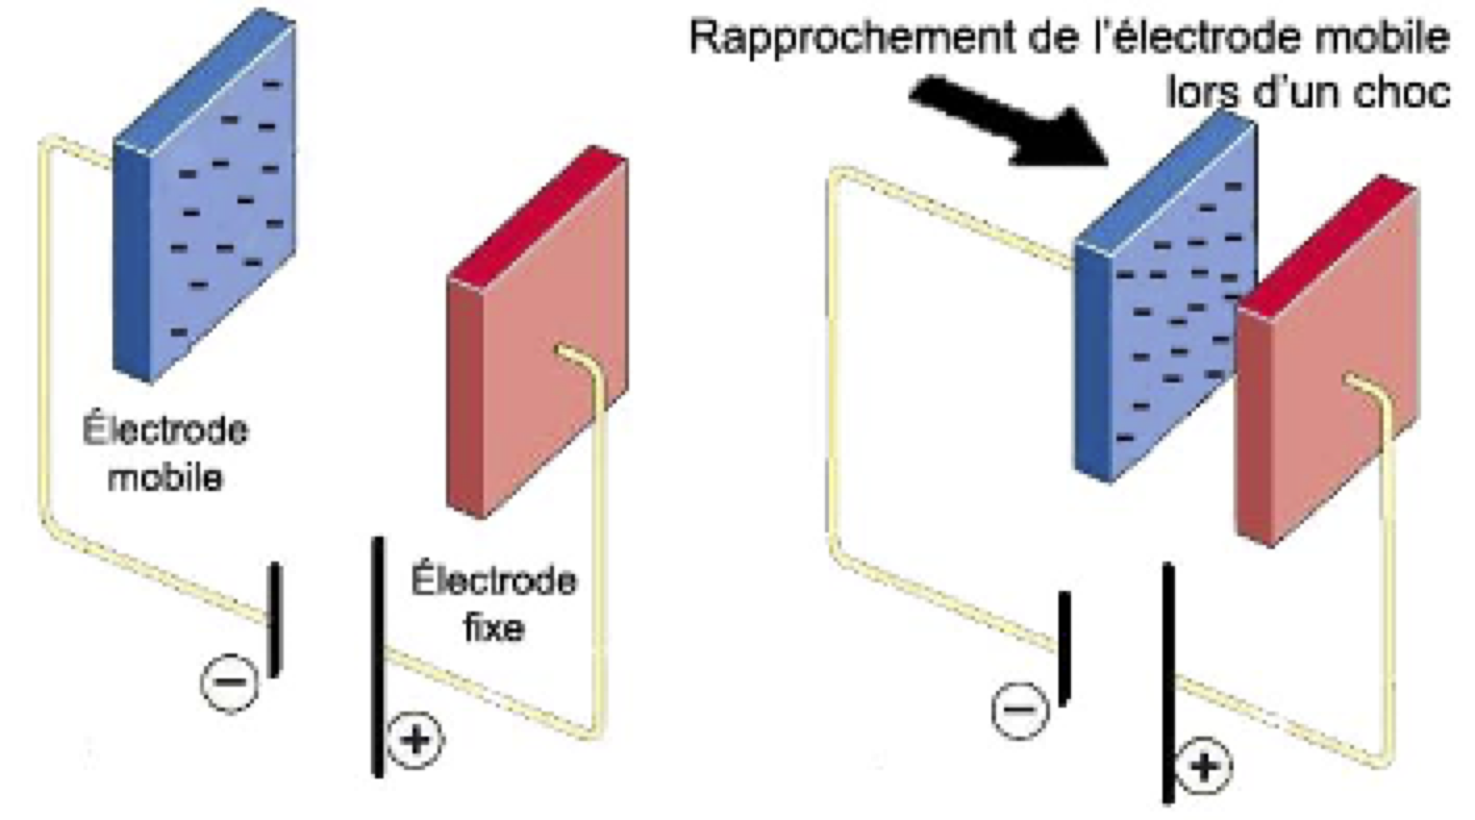
\includegraphics[scale=.7]{Ressources/TSPE_C11_Exercices_Fig1.png}	
	\end{minipage}
\end{minipage}

\vspace{.5cm}
\noindent
\begin{minipage}{.47\linewidth}
	\textbf{Document 4 : Évolution des grandeurs électriques à la mise sous tension de l'accéléromètre}\\
	Courbes d'évolution temporelle de la tension $u_C$ aux bornes de l'accéléromètre et de l'intensité du courant qui le traverse lors de la mise sous tension, lorsque l'accéléromètre est au repos : $C$ = \SI{100}{\pico\farad} et $E$ = \SI{5,0}{\volt}.
\end{minipage}
\begin{minipage}{.5\linewidth}
	\centering
	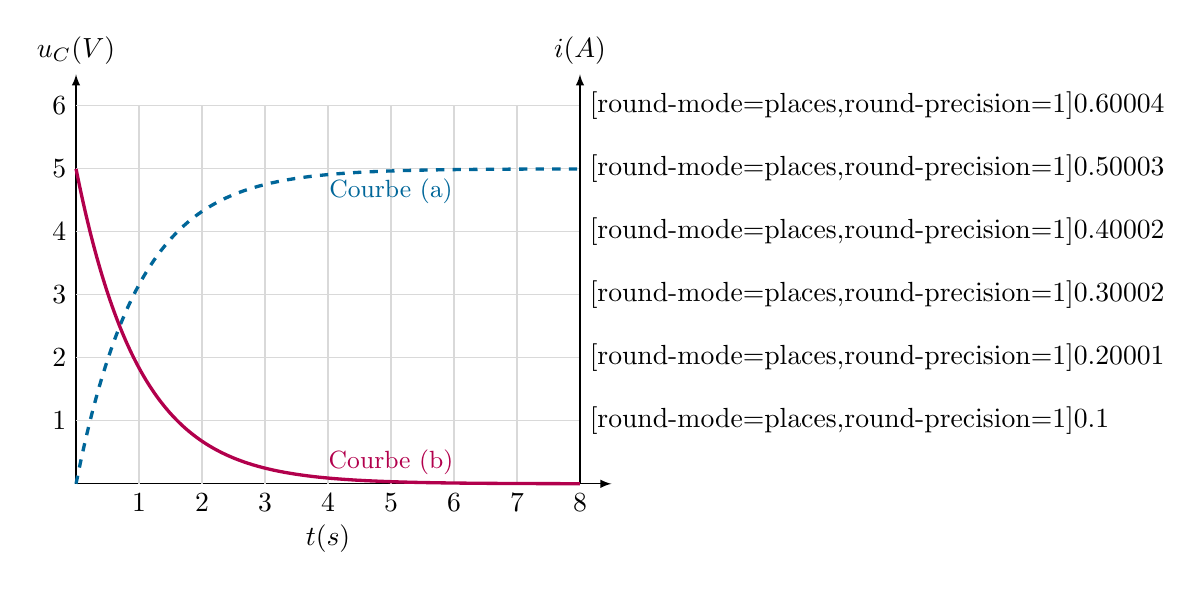
\begin{tikzpicture}[scale=.8]
		\draw[-latex] (0,0) to (0,6.5);
		\draw[-latex] (0,0) to (8.5,0);
		\foreach \k in {1,...,6}{
			\draw[gray!30] (0,\k) to (8,\k);
			\node[left] at (0,\k)  {\k};
			\node[right] at (8,\k)  {\pgfmathparse{0.1*\k} \num[round-mode=places,round-precision=1]{\pgfmathresult}};}
		\foreach \k in {1,...,8}{
			\draw[gray!30] (\k,0) to (\k,6);
			\node[below] at (\k,0)  {\k};}
		
		\draw[-latex] (8,0) to (8,6.5);
		\draw [dashed, domain=0:8,samples = 600,blue!60!green,line width = 1.2pt] plot (\x,{5*(1-exp(-\x/1))});%courbe a
		\draw [domain=0:8,samples = 600,blue!30!red,line width = 1.2pt] plot (\x,{5*exp(-\x/1)});%courbe b
		
		\node[above] at (0,6.5)  {$u_C (V)$};
		\node[above] at (8,6.5)  {$i (A)$};
		\node[below] at (4,-.5)  {$t (s)$};
		
		\node[below,blue!60!green] at (5,5)  {\small Courbe (a)};
		\node[below,blue!30!red] at (5,.7)  {\small Courbe (b)};
		
	\end{tikzpicture}
\end{minipage}

	\textbf{Questions}
\begin{enumerate}
	\item \textbf{Comportement de l'accéléromètre en dehors de chocs}\\
	La mise sous tension de l'accéléromètre revient à fermer l'interrupteur $K$ du montage modélisant le dispositif représenté sur le \textbf{Document 2}.\\
	Le condensateur est déchargé avant la fermeture de l'interrupteur. À la date $t_0$ = \SI{0}{\second}, on ferme l'interrupteur.
	\begin{enumerate}
		\item À l'aide du \textbf{Document 4}, identifier en justifiant qualitativement le courbe correspondant à la tension et celle correspondant à l'intensité.
		\item Délimiter de façon approximative et qualifier les deux régimes de fonctionnement du circuit.
		\item Déterminer graphiquement la valeur du temps caractéristique du dipôle RC et en déduire un ordre de grandeur de la valeur de la résistance $R$.
		\item Déterminer graphiquement sur la figure du \textbf{Document 4} les valeurs de la tension aux bornes du condensateur et de l'intensité du courant en régime stationnaire.
		\item En déduire, en régime stationnaire, la valeur de la charge $q$ du condensateur de capacité $C$.
	\end{enumerate}
	\item \textbf{Déclenchement de l'airbag}
	\begin{enumerate}
		\item D'après le \textbf{Document 1}, indiquer comment se nomment les parties de l'accéléromètre correspondant aux armatures mobile et fixe.\\
		Le rapprochement des deux armatures, provoqué par un choc, entraîne une augmentation de la capacité du condensateur (\textbf{Document 3}). L'objectif de la suite de l'exercice est de comprendre les conséquences de cette variation.\\
		En tenant compte du fait que le temps caractéristique est très faible, on considérera que la valeur de la résistance est nulle.
		\item Parmi les deux propositions suivantes donnant l'expression de la capacité $C$ en fonction de la distance $d$ entre les armatures du condensateur, choisir en justifiant celle qui peut convenir.
		\begin{center}Proposition 1 : $C=k\cdot d$; \hspace{2cm} Proposition 2 : $C=\dfrac{k}{d}$.\end{center}
		\item Donner l'expression de la tension $u_C$ aux bornes du condensateur et de la charge $q$ du condensateur avant le choc, en fonction de $E$.
		\item Justifier que la tension $u_C$ aux bornes du condensateur n'est  pas modifiée par le choc. En déduire que le choc a pour effet de faire augmenter la charge $q$ du condensateur.
		\item Reproduire le schéma du \textbf{Document 3} et indiquer le sens de déplacement des électrons dans le circuit engendré par la variation de charge $q$ du condensateur.
		\item Donner la relation entre la charge $q$ du condensateur et l'intensité $i$ du courant qui le traverse.
		\item Le déclenchement du gonflage de l'airbag est commandé par la détection d'une variation :
		\begin{itemize*}
			\item de tension aux bornes du condensateur
			\item de tension aux bornes du générateur
			\item d'intensité du courant dans le circuit.
		\end{itemize*}
	\end{enumerate}
\end{enumerate}
\end{document}
